\chapter{Design}
\label{ch:design}

This chapter introduces the design choices implemented in our solution in order to overcome the challenges presented in Chapter~\ref{ch:unmaintainability}. We also discuss the implementation of the most critical aspects of these solution. We do not discuss the \acrshort{ui} implementation as it is out of the scope of this thesis. However, we will still discuss its design as it is part of the architecture we present and tackles some important points that make this an interesting issue.

%This chapter presents the challenges encountered creating the system, what the most critical components are and the choices we made to overcome said issues. We first present the components that build up the system, what their responsibility are and the choices that lead us to this design. Then tackle each component one by one, focusing separately on each challenge. Afterwards we combine all the choices and present the final architecture of the system developed.

\section{Components}
\label{sec:components}

Based on our discussion of the challenges in Chapter~\ref{ch:unmaintainability}, we opt for an architecture with components that each have a precise separate concern \cite{Hursch95separationof}. This stems from maintainability driven considerations arising from previous work's code, where components were highly coupled with both the visualization library and the engine \cite{dreuning_visual_2016, duking_potential_2018, kruis_creating_2017, wheeler_virtual_2018}.

The most basic design of our architecture requires two main endpoints, that are \acrshort{vtk} and Unity, a native layer of interfacing between the two and a managed Unity plugin for interfacing native code with the engine. The bare bones implementation was developed by Wheeler et al. \cite{wheeler_virtual_2018}, on which our solution is based. This gives us an infrastructural basement on which our further components then work.

To achieve our goal of full integration of VTK, we cannot rely on hardcoded functions, which would impair the generality of the system, as well as its maintainability. As such, our solution comprises an introspecting component that enables the gathering of metadata on \acrshort{vtk} and thus limits the coupling of the solution to a particular version of \acrshort{vtk}.

On the other hand, the expression of such metadata also needs to be lowly coupled with the particular implementation of \acrshort{vtk}, and as such a component is introduced to enable the generation on-the-fly of UI that fits the I/O operations required to support the development environment. The design of the UI parts themselves is out of the scope of this thesis; we will only discuss its design, which enables the creation of the UIs.

Finally, this generality may come at the price of performance as introspection may be slow and interfacing may not be complete through it, as we discuss in Section~\ref{sec:design-introspection}, and the UI generation may be slow when working with big and complex pipeline filters. A first experiment in Section~\ref{sec:complexity-generality} shows that the performance on the creation of a somewhat complex pipeline using introspection, which yielded promising results. However, these performances may not be enough in all cases to support the use we envision for this software. As such, to enable users to enhance their experiences, both  tailored, more user-friendly UIs as well as focused and efficient adapters that create a direct link between the infrastructure and \acrshort{vtk} features are introduced in the architecture.

The final architecture is composed of a total of six components, as shown in Figure~\ref{fig:high-level-architecture}:

\begin{itemize}
    \item An \textbf{Infrastructure Layer} which acts as bridge between \acrshort{vtk} and Unity;
    \item A \textbf{\acrshort{vtk} Interfacing Layer}, comprised of an \textbf{Adapter Interface}, which uses custom made code by the user to interface with \acrshort{vtk}, and an \textbf{Introspection Interface}, which uses introspection over \acrshort{vtk} to access its features;
    \item A \textbf{Unity Managed plugin} which allows Unity to access the functionality exposed by the \textit{Infrastructure Layer};
    \item A \textbf{Unity UI Library}, comprised of a \textbf{UI Toolbox}, which is made of custom UIs created to tailor specific usages, and a \textbf{UI Composer}, which uses a minimal set of UI components to generate UIs on-the-fly.
\end{itemize}

\begin{figure}
    \centering
    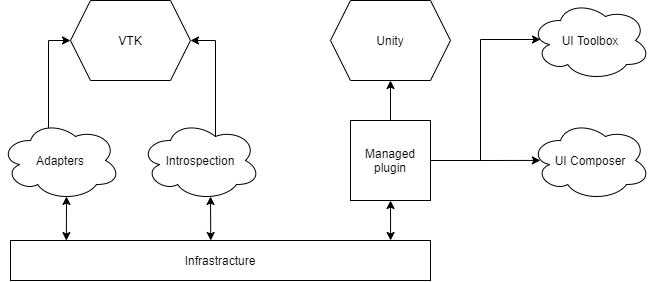
\includegraphics[width=\textwidth]{pictures/Architecture-high-level-transparent.png}
    \caption{Components and their interconnections.}
    \label{fig:high-level-architecture}
\end{figure}

\section{Infrastructure}
\label{sec:design-infrastructure}

The infrastructure layer is the component responsible for allowing interaction between all other parts of the system. Its main job is to give a common entry-point to the \acrshort{vtk} interfaces and decide which to call, acting as a dispatcher. As this is the critical point of the system where communication flows, it is also the one that mostly affects parallelization and distribution capabilities. Thus, the calls should be as little blocking as possible, allowing flows to stop only at endpoints and not in the middleware.

Wheeler et al.'s VtkToUnity \cite{wheeler_virtual_2018} already partly implements this infrastructure layer and already exposes part of the \acrshort{vtk} interface as well. Unfortunately, their calls are highly blocking, as once the C++ native code executes, the Plugin calls each \verb|lock()| on the API and thus parallel calls are impossible. On the other hand, the plugin achieves decent performances that fall within the Unity guidelines for \acrshort{vr} \cite{unity_vr_2020}, while allowing for good maintainability and extension possibilities.

As such, we base the infrastructure layer on a refactoring of the VtkToUnity plugin which aims at the following results:

\begin{enumerate}
    \item Decoupling of the communication and dispatching from the interfacing responsibilities;
    \item Refactoring the interfacing code in adapters that constitute the foundation of the adapter-based interfacing;
    \item Move as much business logic of the infrastructure in non-blocking calls, preferably with no blocking at the infrastructure layer;
    \item Move blocking logic at interface level.
\end{enumerate}

%As we expect the interfacing to be slower, especially with the introspection component, the infrastructure layer will also have a cache system to store and retrieve the latest hits and directly call the precise function rather than going through with the introspecting dispatch system.

We use the same approach as in the VtkToUnity plugin to create the C++ native plugin and its interfacing with Unity. Our implementation is then reduced to the minimal API necessary to use the \acrshort{vtk} functionality expressed by the interface mechanisms described in Section~\ref{sec:design-interfaces}. Our objective is to make the calls as general as possible, giving the user the most liberty and access as possible. For the naming and implementation, we follow a similar design as the Python/C API \cite{python_c_api}. The interface is comprised of the following methods:

% TODO: review the functions and update to new interface
\begin{itemize}[leftmargin=1.5truecm]
    \setlength{\itemindent}{-1truecm}
    \item[] \verb|AddVtkObject(objectName, rgbaColour, wireframe, objectId)| takes as input a string representation of the \acrshort{vtk} object to instantiate, the rendering colour and a flag to show the wireframe, and returns the objectId of the shape, which is its index in the object registry that the infrastructure layer keeps;
    \item[] \verb|GetVtkObjectProperty(objectId, propertyName, returnValue)| takes as input the object's index in the registry and the name of the property, accesses the \acrshort{vtk} interface as described in Section~\ref{sec:design-interfaces}, and returns the string representation of the value;
    \item[] \verb|SetVtkObjectProperty(objectId, propertyName, newValue)| takes as input the object's index in the registry, the name of the property to change and the new value and accesses the \acrshort{vtk} interface to set the object's attribute to the new value;
    \item[] \verb|GetVtkObjectDescriptor(objectId)| takes as input the object's index in the registry, and returns a string representation of the attributes of the object; this is used then in the UI composer to generate the UI for manipulating the objects;
    \item[] \verb|RemoveVtkObject(objectId)| takes as input the object's index in the registry, and deletes it.
\end{itemize}

\section{VTK Interfaces}
\label{sec:design-interfaces}

The core feature of our system is its ability to access \acrshort{vtk} and expose it fully to the \acrshort{vr} development environment. To achieve this, while keeping the system easily maintainable and performing, we use a two way access system. The first access route uses a lookup to check whether custom adapters exist that can satisfy the request from the caller, while the second uses introspection capabilities on the library to find the appropriate method, function or class that can satisfy the request.

We discuss both access tiers and how each of them is designed. Both these subsystems are intended to be separate services that the main architecture can either directly access when running in a stand-alone version on the users PC, or can be distributed on a network and be accessed through distribution engines such as DtCraft \cite{huang2017dtcraft} or Boost::MPI \cite{schaling2011boost}.

\subsection{Adapters}
\label{sec:design-adapters}

The first access tier for \acrshort{vtk} is a set of custom adapters that users can define, expand and modify and get built with the solution. These adapters have the objective of allowing the user to customize their system and tailor it to their needs. The user can define different ways in which the native plugin interacts with \acrshort{vtk}. Particular use cases for adapters are:

%TODO: implementation of other two use cases
\begin{enumerate}
    \item The creation of custom loggers for diagnostics and flow analysis;
    \item Implementation of \textit{templates} at native level that enable faster instantiation and define their own parameters and routines;
    \item Implementation of custom algorithms that compound \acrshort{vtk} features.
\end{enumerate}

The adapters are Singleton instances that define first and foremost a unique string identifying which component they are adapting. Such ID represents the name of the object the code adapts. For instance, an adapter for the  source class \verb|vtkConeSource| should be identified by the class' name. Furthermore, each adapter has to implement access methods for getting descriptions of what attributes the class has, getting the values of each of those attributes and setting such values as well. 

Optionally, the adapter can implement rendering information in case the adapter is not for a specific \acrshort{vtk} class but for a template or custom algorithm, in which case information is needed on how to render and update the objects generated by the adapter.

The main driver behind adapters is to make the solution maintainable as well as generic. We do not foresee all potential uses of the adapters, as it is not our objective. Their implementation is kept to the bare minimum and some use cases are presented which are, to us, the most obvious. We set out to not limit the potential for these component, and require the implementation of what is needed to make it work.

In order to implement the defined adapters, we first define a basic adapter class which is used for only use case number 1, i.e. the adapting of \acrshort{vtk} defined objects. This class does not define rendering and update information, as these are already defined by \acrshort{vtk}. We implement \verb|VtkAdapter| as shown in listing~\ref{lst:vtkadapter}

\begin{figure}
    \centering
    \begin{cpp}[label=lst:vtkadapter,caption={vtkAdapter class}]
class VtkAdapter
{
public:
	template <typename T> using getter = std::stringstream(T::*)(vtkSmartPointer<vtkActor>);
	template <typename T> using setter = void (T::*)(vtkSmartPointer<vtkActor>, LPCSTR);

	virtual ~VtkAdapter() { }

	inline LPCSTR GetAdaptingObject() {
		return m_vtkObjectName;
	}

	virtual void SetAttribute(vtkSmartPointer<vtkActor> actor, LPCSTR propertyName, LPCSTR newValue) = 0;
	virtual void GetAttribute(vtkSmartPointer<vtkActor> actor, LPCSTR propertyName, char* retValue) = 0;
	virtual void GetDescriptor(char* retValue) const = 0;

protected:
	LPCSTR m_vtkObjectName;

	VtkAdapter(LPCSTR vtkObjectName) { 
		m_vtkObjectName = vtkObjectName;
	};
};
    \end{cpp}
\end{figure}

The class has a unique identifier in the form of a \verb|LPCSTR| (Long Pointer to Const STRing) which is to be set when instantiating the adapter. The class also carries with it a descriptor of the \acrshort{vtk} class that specifies what attributes the class has and what is their type. This descriptor is used by the Unity Managed plugin as we discuss in Section~\ref{sec:design-uicomposer}.

Alongside these functions, there are two templates that define the types of \verb|getter| and \verb|setter| methods used by adapters. These functions take as input a pointer to the actor that renders the \acrshort{vtk} object and the first returns a string representation of the value of the attribute while the second takes a further argument that is the new value to which attribute is to be set.

The generic calls for getting and setting attributes are respectively \verb|GetAttribute| and \verb|SetAttribute|. These functions act as dispatchers for the particular operations, that can either be directly implemented into the function but, as good practice, we later show an example of how we recommend these adapters should be implemented.

The actual attribute to change is encoded in a \verb|LPCSTR| that contains the name of the attribute exactly as written in the C++ code. A difference from the \verb|GetAttribute| generic call and the particular \verb|getter| template is that the return value is not returned but a specific parameter acts as return buffer, as this value is not to be used inside the C++ native code but to be sent through to the C\# interface in Unity.

Alongside the adapters, the \verb|VtkAdapterUtility| provides the access point for the register of the adapters. This allows to couple adapters to a single point of entry and masks the adapters to the infrastructure layer, making it easy to execute on a separate service. The implementation of this class is generated by a Python script at build time, available in Appendix~\ref{apx:generate-register}. The interface of the utility is shown in Listing~\ref{lst:vtkadapterutility}.

\begin{figure}
    \centering
    \begin{cpp}[label=lst:vtkadapterutility,caption={VtkAdapterUtility interface}]
class VtkAdapterUtility
{
public:
	static VtkAdapter* GetAdapter(LPCSTR vtkAdaptedObject);

private:
	static const std::unordered_map<LPCSTR, VtkAdapter*> s_adapters;
};
    \end{cpp}
\end{figure}

As visible, the adapter only exposes the function \verb|GetAdapter| that returns the implementation of the adapter for the unique ID requested if such object exists, \verb|NULL| otherwise. The adapters are stored in an unordered map, as it has faster access times than the ordered counterparts \cite{stdunord16, stdmapcp55} on the average case. This depends on the hashing function, but as we use default types for keys and we do not replicate them, the average case is almost certainly guaranteed. The map is populated on instantiation and the entries are generated as Singletons, as shown in Listing~\ref{lst:adaptersmap}.

\begin{figure}
    \centering
    \begin{cpp}[label=lst:adaptersmap,caption={Example of adapters register instantiation.}]
const std::unordered_map<LPCSTR, VtkAdapter*> VtkAdapterUtility::s_adapters =
{
	{ Singleton<VtkConeSourceAdapter>::Instance()->GetAdaptingObject(), Singleton<VtkConeSourceAdapter>::Instance() },
	// More adapters...
};
    \end{cpp}
\end{figure}

\subsection{Introspection}
\label{sec:design-introspection}

% As one of the objectives is to make the software less dependant on the \acrshort{vtk} version, a component with introspection capabilities is introduced to gather the necessary information on the \acrshort{vtk} implementation used. As most of the native implementation of the plugin is written in C++, we can either find a way to introduce introspection capabilities in C++ or use a language which both has a \acrshort{vtk} wrapper available and has such tools.

% For the first option, some research has been carried out and the results are incomplete \cite{tyng1998nonintrusive} or introduce non-trivial overheads \cite{bayser2012rtti}, and in both cases would mean the introduction of further maintainability issues. The second option is not better either when it comes to new couplings, and we introduce a third language to the software as well as potential libraries necessary for communication.

% As previous solutions already exist that offer some capabilities as we require for \acrshort{vtk} in Python \cite{dreuning_visual_2016}, we opt for an embedded design, even though it may not be the best performance-wise, it allows us to use established libraries with decent communities supporting them, whereas most C++ introspection extensions offer limited support.

As we discussed in Section~\ref{sec:complexity-generality}, solutions already exist that implement introspective systems to access VTK in Python. In particular, we modify and extend the Python scripts from Dreuning's solution in order to make use of its \verb|ClassTree|. The issue we find with this implementation is that it is limited to \verb|vtkAlgorithm| classes, and as such leaves out a chunk of the features of the VTK. As extending these scripts is out of the scope of this thesis, we instead introduce a feature to overcome this limitation that would nevertheless be implemented, i.e. the ability to pipe the result of a VTK call to other calls. This does not allow the user to instantiate objects of classes that are not \verb|vtkAlgorithm|, however it allows already for a big part of the left out features to be accessed.

From Dreuning's solution we adapt the \verb|ClassTree| implementation in order to strip it of its UI related code, as well as the \verb|PipelineObject|, which we use as the introspective wrapper for the \acrshort{vtk} objects we instantiate to hold the getter and setter calls. A further script has been produced to facilitate the calls from C++, exposing the required features for: (a) creating a (wrapped) \acrshort{vtk} object and return the C++ object's address; (b) getting the description of a \acrshort{vtk} object, i.e. its attributes and their types, used by the Composer to generate UIs on-the-fly; (c) get the value of a \acrshort{vtk} object's attribute; (d) set the value of a \acrshort{vtk} object's attribute; and (e) delete the wrapper's information once the \acrshort{vtk} object gets deleted in the environment. 

In order to access the Python scripts from the C++ native plugin, we embed the Python 3.7 interpreter in the C++ implementation. This is achieved by initializing the interpreter as part of the process, using a subset of the software's memory to run Python. This, combined with the ability to wrap the C++ VTK objects using the \verb|vtkPythonUtils| class into Python and then access them back again, allows us not to worry about synchronizing memory and processes, boosting both memory and time performances.

The implementation instantiates a \verb|Introspector| class from Python, using it as access-point for the introspective methods. Using the \verb|PyObject_CallMethod| we are able to use the methods of the \verb|Introspector|, starting with \verb|createVtkObject| which instantiates a wrapped VTK object, using the class name, that carries the information of the getter and setter methods of the \verb|vtkAlgorithm| class. These wrapped objects, that we will now call \textit{nodes}, are registered in a structure that maps the pointer of the C++ object to its wrapped Python counterpart, for fast lookup access \cite{stdunord16}. The C++ interface exposes calls that allow, having the node available, to call getters, setters, to execute the VTK update of the object, retrieve the output port, delete the object, execute a generic or piped call. This last one means that you can execute, for example, \verb|object.GetOutput().GetCenter()| with a single access to the \verb|Introspector| and use non introspectable objects as intermediate values, expanding the possible calls that the plugin can execute.

To avoid ambiguity when calling these methods, and to avoid passing excessive data through the Unity native interface, the methods that retrieve values from the \verb|Introspector| use a postfix notation to determine whether the call is to return a native value that can easily be parsed to and from a string representation (\verb|_AsString|), an id of a VTK object (\verb|_AsVtkObject|), or either if the result is to be discarded or the method being called has \verb|void| return type (\verb|_AsVoid|).

When calling any method that uses parameters of generic types, we use a similar convention as the Python/C API so to make the maitainability of the code easier, as these are strictly intertwined and usually used alongside. As such, calls are structured as follows: the first parameter is the pointer to the object on which the method is to be called, the second parameter is the name of the method to be called, or a specifier that acts as a dispatching value (i.e. dispatching either to \verb|SetInputConnection| or \verb|SetSourceConnection|), third is the string format of the following parameters (e.g. a method that has three doubles as parameters would have as format \verb|"fff"|), and finally a vector containing the parameters. Special treatment is reserved for the \verb|"O"| object parameters that are first past as string representation of integer values, then parser to integers by the infrastructure layer, which represents the id of the VTK object in the registry, and finally two vectors are sent to the introspection layer, one with the \verb|vtkObjectBase *| objects and the other with the rest of the parameters.

A complete description of the formatting values see Table~\ref{tab:format-values}, while the interface of the introspection layer is documented in Appendix~\ref{apx:api}

\begin{table}[ht!]
    \centering
    \begin{tabulary}{.9\textwidth}{LL}
    \multicolumn{1}{c}{\textbf{Symbol}} & \multicolumn{1}{c}{\textbf{Meaning}} \\ \hline
    O & A VTK object. The value from the Managed plugin is the ID of the object in the infrstructure layer's registry. The Introspection layer receives the pointer to the VTK object. \\
    d                                   & A C integer or long value.           \\
    f                                   & A C float or double value.           \\
    s                                   & A C char or LPCSTR value.            \\
    b                                   & A C++ bool value.                    \\
    \%\# & is any of the previous symbols, \# is the number of values. It represents a tuple of values, e.g.: f3 corresponds to (fff) in the Python/C API.
    \end{tabulary}
    \caption{Format symbols used in the calls to the plugin.}
    \label{tab:format-values}
\end{table}

%\begin{itemize}[leftmargin=1.5truecm]
%    \setlength{\itemindent}{-1truecm}
%    \item[] \verb|createVtkObject(objectName)| takes as input the name representation of the \acrshort{vtk} object class, and returns a (wrapped) \acrshort{vtk} object;
    
%\end{itemize}

% In order to use this code from the C++ implementation, we embed the Python interpreter in the software. Fortunately, this is a use case covered in the Python/C API documentation\footnote{\url{https://docs.python.org/3.6/extending/embedding.html}}. While this solution already achieves a lot for our software, we handle a lot of objects and all the instantiation and de-instantiation of these objects requires a lot of verbose code. A few options are available to reduce the complexity of the code, in particular we consider the \verb|vtkPythonInterpreter| module from \acrshort{vtk} itself and the Boost::Python library that exposes a simplified version of the Python/C API for both embedding and extending \cite{abrahams2003building, schaling2011boost}.

% Both present pros and cons, and in both cases impact the maintainability of the system. The \acrshort{vtk} module allows us to not couple our solution to further software, keeping all the external code encapsulated in \acrshort{vtk}. This is though a limited solution, as it exposes a very limited set of functionality of the Python/C API, based on previous uses of Python embedding in native \acrshort{vtk} software.

% On the other hand, Boost is a more versatile library, which exposes a general purpose API for Python/C extending and embedding. Even though more powerful than the \acrshort{vtk} module, it still is not complete, and the Python/C API still needs to be used in particular situations. Furthermore, it presents some conflicts with how the Python/C API is intended to be used, e.g. the \verb|Py_Finalize()| should not be called when using Boost::Python. Adding the fact that this introduces a further coupling with external software, presents multiple challenges towards the maintainability of our solution.

% Given these considerations, we opt for the integrated module of \acrshort{vtk} as to drive down unmaintainability factors.

\section{Managed Plugin}
\label{sec:design-managed-plugin}

The integration of VTK with Unity makes use of both a native plugin, which we already discussed, and a managed plugin, which is the focus of this section. In particular, this part of the system is responsibile for making the native plugin API more user-friendly, and connecting the rendering cycles of the two rendering contexts. The setup is almost identical to the VtkToUnity plugin, with a different API for VTK.

The basic API of the managed plugin is identical to the native plugin API, with the exception of the usage of the \verb|Marshal|, a .NET library used to work with unmanaged memory areas. In Unity, this library is used in particular to handle passing paramters back and forth between the managed and native parts of the environment, like defining how strings have to be handled passing down to C++. In our implementation we use this exclusively to specify strings to be handled as long pointer strings, as we represent them as \verb|LPCSTR| (Long-Pointer Constant STRing) in our C++ code.

As a further design discussion, we present now the Toolbox and Composer components that are part of the managed plugin. As the UI is out of the scope of this thesis, we will not discuss particular implementations of these components, as they will be presented in a separate thesis. Designing these components, we mirror our approach to accessing VTK, as our drivers remain the same. In particular, the Toolbox is the component that mirrors the Adapters registry, while the Composer mirrors the Introspector.

\subsection{Toolbox}
\label{sec:design-toolbox}

As UIs are in general more complex than accessing introspectively a library, as they are made of more components and constrained by interaction and usage limits that depend on the device being used, the environment, the input devices and so on, the ability to introduce custom-tailored UI components is necessary. Thus, we propose the usage of a registry of UI prefabs developed in Unity as first-tier access to the UI of the environment.

A registry mapping from the classname to the prefab factory \verb|IComponentFactory| acts as the access-point for the UI instantiation. When a part of the pipeline is created, the \verb|FactoryManager| first checks the registry to check whether a factory for the entire UI exists. If this exists, the factory is called and a \verb|Create| function generates the UI based on the prefab. The UI is then linked to the particular part of the pipeline by the manager in order to keep track of the changes and to avoid the changes being either lost or set to the wrong VTK object. This is also to have the UI ready but not shown, and only made visible through \verb|Show| when necessary and hidden through \verb|Hide| when changing focus.

% TODO: write more

\subsection{Composer}
\label{sec:design-uicomposer}

If the Toolbox fails, a generic system to generate UIs gets called. This requires more resources and time to execute, as it takes the descriptor of the VTK object, which maps the names of the attributes to their types, and then creates a minimal UI with this information. The Composer uses a registry of minimal components that are part of the environment that implement interfaces to edit native simple values, e.g. integers, decimals, booleans, strings and so on. These components are also registered with the Toolbox, for faster access.

The generated components this way are then used to instantiate a \verb|ComposedUI| object, that contains the information of the different parts that make the UI and then add this to the Composer's registry, acting as a \verb|IComponentFactory| for later calls of the \verb|FactoryManager| on the same classname to avoid generating the same factory twice.

In order to accelerate and expand the Composer's ability, the mappings are not hardcoded; the Composer still uses the Toolbox as a lookup for the basic parts used to generate the UI, and thus custom-tailored basic UIs can be added to the Toolbox to override the natively implemented ones.

% TODO: write more